\chapter{Molekul Organik: Kerangka dan Nama}\label{ch:g11:organic-skeletons}

Korek api gas sekali pakai berisi butana, yang cair di bawah tekanan;
tabung kompor kemah yang dibawa mendaki gunung bersalju berisi propana,
atau \omterm{def:g6:pure-substances-and-mixtures:mixture}{campuran} yang lebih kaya propana. Keduanya hanya tersusun atas \omterm{def:g7:atoms-and-molecules:atom}{atom}
karbon dan hidrogen, dan keduanya termasuk keluarga yang sangat besar:
\omterm{def:g7:atoms-and-molecules:molecule}{molekul-molekul} yang dibangun di atas kerangka \omterm{def:g7:atoms-and-molecules:atom}{atom} karbon. Jutaan
\omterm{def:g7:atoms-and-molecules:molecule}{molekul} seperti itu telah dikenal. Untuk membicarakannya, para ahli
kimia memerlukan cara untuk menggambarnya dengan cepat dan menamainya
tanpa keraguan.

\begin{recall}
Karbon membentuk empat \omterm{def:g10:lewis-and-shape:covalent-bond}{ikatan kovalen} dan hidrogen satu; di sekeliling
\omterm{def:g7:atoms-and-molecules:atom}{atom} karbon dengan empat ikatan tunggal, ikatan-ikatan itu mengarah ke
sudut-sudut sebuah tetrahedron, dengan sudut sekitar \ang{109.5}
(\cref{ch:g10:lewis-and-shape}).
\end{recall}

\begin{omfigure}
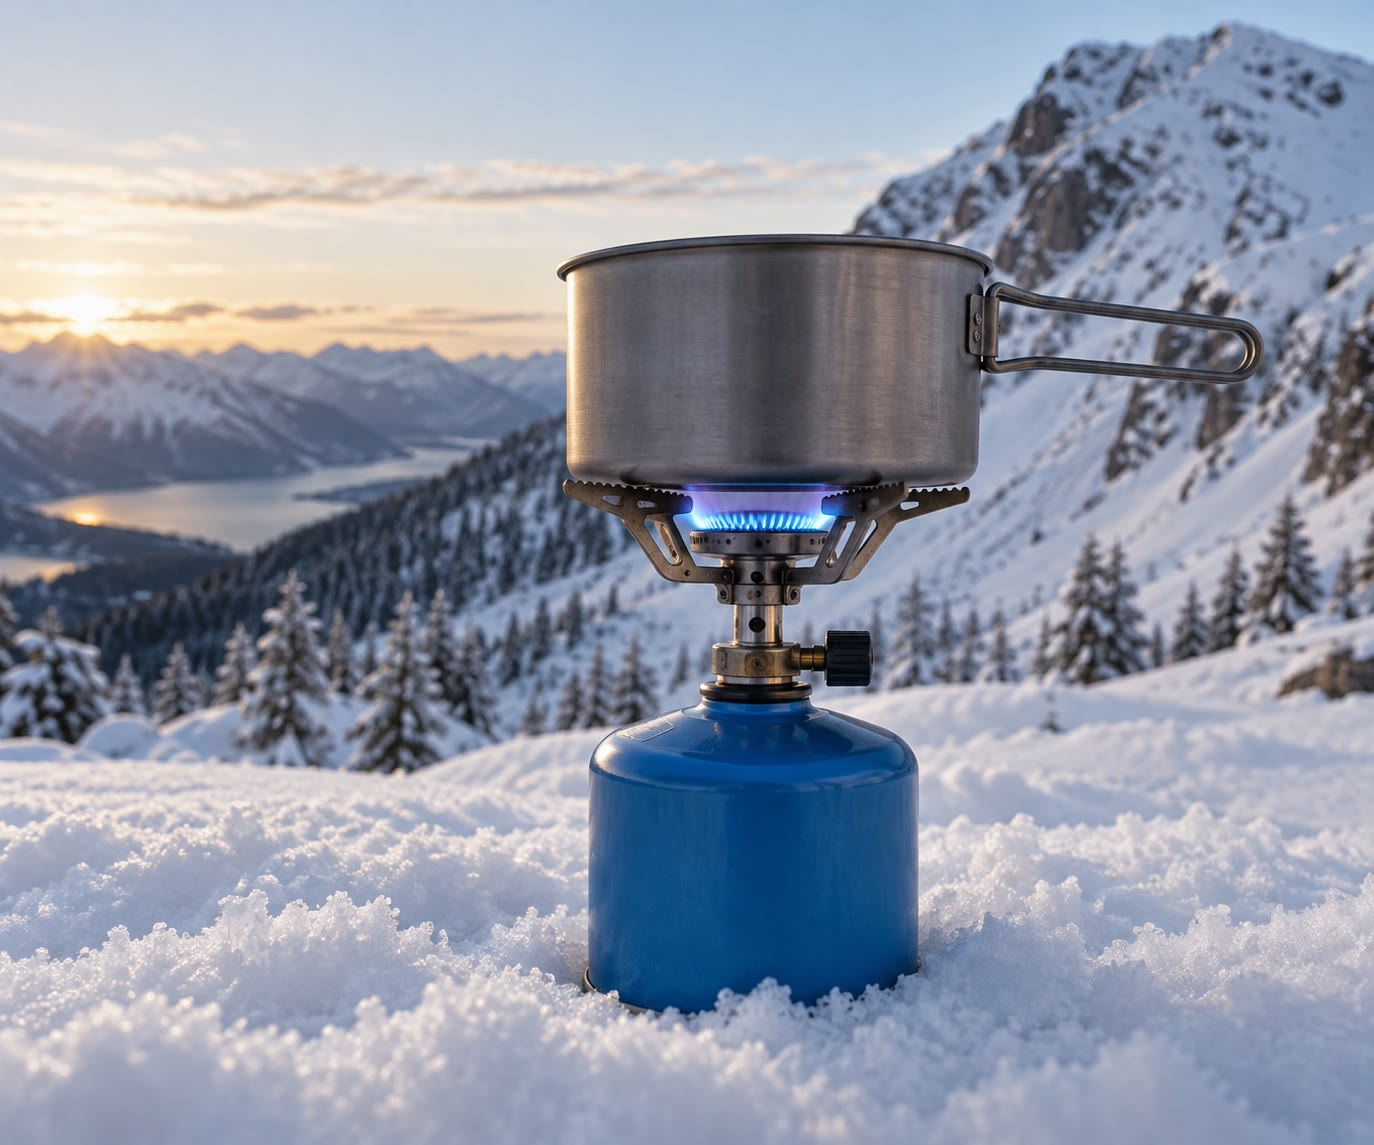
\includegraphics[width=0.48\linewidth]{images/book1/ai/g11-camping-cartridge.jpg}

{\small Kompor kemah di tengah salju, membakar gas yang tersusun atas
karbon dan hidrogen.}
\end{omfigure}

\section{Rumus molekul organik}

\begin{definition}[Senyawa organik]\label{def:g11:organic-skeletons:organic}
Yang disebut \emph{senyawa organik}\index{senyawa organik} adalah
senyawa yang \omterm{def:g7:atoms-and-molecules:molecule}{molekulnya} dibangun di atas kerangka \omterm{def:g7:atoms-and-molecules:atom}{atom-atom} karbon yang
terikat satu sama lain dan dengan \omterm{def:g7:atoms-and-molecules:atom}{atom-atom} hidrogen, mungkin pula
dengan \omterm{def:g7:atoms-and-molecules:atom}{atom} lain seperti oksigen dan nitrogen. (Karbon dioksida, karbon
monoksida, dan karbonat secara tradisional tidak dimasukkan.)
\end{definition}

\begin{definition}[Empat jenis rumus]\label{def:g11:organic-skeletons:formulas}
Sebuah \omterm{def:g7:atoms-and-molecules:molecule}{molekul} dapat dituliskan dengan empat cara:
\begin{itemize}
  \item \emph{rumus molekul}\index{rumus molekul} hanya menyatakan
        banyaknya \omterm{def:g7:atoms-and-molecules:atom}{atom} setiap unsur, seperti \ce{C4H10};
  \item \emph{rumus struktur}\index{rumus struktur} memperlihatkan
        setiap \omterm{def:g7:atoms-and-molecules:atom}{atom} dan setiap ikatan;
  \item \emph{rumus struktur ringkas}\index{rumus struktur ringkas}
        memperlihatkan ikatan-ikatan antaratom karbon dan mengelompokkan
        \omterm{def:g7:atoms-and-molecules:atom}{atom-atom} hidrogen dengan karbonnya, seperti
        \ce{CH3-CH2-CH2-CH3};
  \item \emph{rumus kerangka}\index{rumus kerangka} hanya menggambar
        ikatan-ikatan kerangka karbon sebagai garis zig-zag: setiap ujung
        dan setiap sudut adalah \omterm{def:g7:atoms-and-molecules:atom}{atom} karbon, \omterm{def:g7:atoms-and-molecules:atom}{atom-atom} hidrogen pada
        karbon tidak digambar, dan setiap \omterm{def:g7:atoms-and-molecules:atom}{atom} lain (beserta \omterm{def:g7:atoms-and-molecules:atom}{atom-atom}
        hidrogennya) dituliskan.
\end{itemize}
\end{definition}

\begin{omfigure}
\setchemfig{atom sep=1.45em}
\renewcommand{\arraystretch}{1.6}
\small
\begin{tabular}{@{}l@{\quad}c@{\quad}c@{}}
 & butana & 2-metilpropana \\
\omterm{def:g7:atoms-and-molecules:molecule}{molekul} & \ce{C4H10} & \ce{C4H10} \\[4pt]
struktur &
\chemfig{H-C(-[2]H)(-[6]H)-C(-[2]H)(-[6]H)-C(-[2]H)(-[6]H)-C(-[2]H)(-[6]H)-H} &
\chemfig{H-C(-[2]H)(-[6]H)-C(-[6]H)(-[2,1.5]C(-[1]H)(-[3]H)(-[2]H))-C(-[2]H)(-[6]H)-H} \\[10pt]
struktur ringkas & \ce{CH3-CH2-CH2-CH3} &
\chemfig{CH_3-CH(-[6]CH_3)-CH_3} \\[14pt]
kerangka & \chemfig{-[:30]-[:-30]-[:30]} & \chemfig{-[:30](-[:90])-[:-30]} \\
\end{tabular}

{\small Keempat rumus butana dan 2-metilpropana. Pada \omterm{def:g11:organic-skeletons:formulas}{rumus kerangka},
setiap ujung dan setiap sudut garis adalah \omterm{def:g7:atoms-and-molecules:atom}{atom} karbon: masing-masing
empat.}
\end{omfigure}


\begin{example}[Membaca rumus kerangka]\label{ex:g11:organic-skeletons:reading}
Pada \omterm{def:g11:organic-skeletons:formulas}{rumus kerangka} butana, garis zig-zag memiliki dua ujung dan dua
sudut: empat \omterm{def:g7:atoms-and-molecules:atom}{atom} karbon. Setiap karbon ujung digambar dengan satu
ikatan, sehingga mengikat tiga \omterm{def:g7:atoms-and-molecules:atom}{atom} hidrogen (\ce{CH3}); setiap sudut
digambar dengan dua ikatan, sehingga mengikat dua (\ce{CH2}). Setiap
karbon memiliki empat ikatan seluruhnya, sehingga kita memperoleh kembali
\ce{C4H10}.
\end{example}

\section{Rantai karbon}

Kerangka karbon sebuah \omterm{def:g7:atoms-and-molecules:molecule}{molekul} dapat berupa rantai \emph{lurus}, setiap
karbon terikat pada paling banyak dua karbon lain, seperti pada butana;
rantai \emph{bercabang}, dengan sedikitnya satu karbon terikat pada tiga
atau empat karbon lain, seperti pada 2-metilpropana; atau \emph{cincin},
seperti pada sikloheksana, \ce{C6H12}, yang \omterm{def:g11:organic-skeletons:formulas}{rumus kerangkanya} berupa
segi enam. Garis zig-zag dipakai untuk rantai karena ikatan-ikatan yang
sebenarnya di sekeliling setiap karbon membentuk sudut sekitar
\ang{109.5}, bukan \ang{180}: rantai yang ``lurus'' sebenarnya berupa
zig-zag di dalam ruang.

\begin{omfigure}
\setchemfig{atom sep=1.9em}
\begin{tabular}{ccc}
\chemfig{-[:30]-[:-30]-[:30]-[:-30]-[:30]} &
\chemfig{-[:30](-[:90])-[:-30]-[:30](-[:90])-[:-30]} &
\chemfig{*6(------)} \\[4pt]
\small lurus: heksana & \small bercabang: 2,4-dimetilpentana &
\small cincin: sikloheksana \\
\small \ce{C6H14} & \small \ce{C7H16} & \small \ce{C6H12}
\end{tabular}

{\small Tiga kerangka karbon, dalam \omterm{def:g11:organic-skeletons:formulas}{rumus kerangka}.}
\end{omfigure}

\section{Alkana dan namanya}

\begin{definition}[Alkana, gugus alkil]\label{def:g11:organic-skeletons:alkane}
Yang disebut \emph{alkana}\index{alkana} adalah senyawa karbon dan
hidrogen yang kerangkanya berupa rantai (lurus atau bercabang, bukan
cincin) dengan ikatan tunggal saja; \omterm{def:g11:organic-skeletons:formulas}{rumus molekulnya} \ce{C_{n}H_{2n+2}}.
Yang disebut \emph{gugus alkil}\index{gugus alkil} adalah sisa sebuah
alkana jika satu \omterm{def:g7:atoms-and-molecules:atom}{atom} hidrogennya dilepas, sehingga gugus itu dapat
dipasang pada sebuah rantai: metil \ce{-CH3}, etil \ce{-CH2-CH3}.
\end{definition}

\begin{omfigure}
\begin{tabular}{rlcrlc}
\hline
$n$ & nama & rumus & $n$ & nama & rumus \\
\hline
1 & metana & \ce{CH4}    & 6  & heksana & \ce{C6H14} \\
2 & etana  & \ce{C2H6}   & 7  & heptana & \ce{C7H16} \\
3 & propana & \ce{C3H8}   & 8  & oktana & \ce{C8H18} \\
4 & butana  & \ce{C4H10}  & 9  & nonana & \ce{C9H20} \\
5 & pentana & \ce{C5H12}  & 10 & dekana & \ce{C10H22} \\
\hline
\end{tabular}\par\medskip

{\small Sepuluh \omterm{def:g11:organic-skeletons:alkane}{alkana} rantai lurus yang pertama. Nama rantai dengan $n$
\omterm{def:g7:atoms-and-molecules:atom}{atom} karbon adalah akar kata yang sama diikuti \emph{-ana}; \omterm{def:g11:organic-skeletons:alkane}{gugus
alkilnya} mengganti \emph{-ana} dengan \emph{-il} (metil, etil,
propil\dots).}
\end{omfigure}

\begin{method}[Menamai alkana]\label{met:g11:organic-skeletons:naming}
\begin{enumerate}
  \item Carilah rantai \omterm{def:g7:atoms-and-molecules:atom}{atom} karbon yang terpanjang: rantai itu memberikan
        nama induknya (pentana, heksana\dots).
  \item \omterm{def:g7:atoms-and-molecules:atom}{Atom-atom} yang tidak termasuk rantai itu membentuk gugus-gugus
        alkil yang terpasang padanya, yaitu substituen.
  \item Berilah nomor rantai utama dari ujung yang memberikan nomor
        terkecil kepada substituen-substituennya.
  \item Tuliskan setiap substituen dengan nomornya (letaknya pada
        rantai), menurut urutan abjad, di depan nama induk; gugus yang
        berulang diberi awalan di-, tri-, tetra-, dengan satu nomor
        untuk masing-masing. Nomor dipisahkan dengan koma, nomor dan kata
        dengan tanda hubung.
\end{enumerate}
\end{method}

\begin{omfigure}
\begin{tikzpicture}[font=\small, x=0.9cm, y=0.9cm]
  % main chain of 5, zigzag; methyls on C2 and C3
  \coordinate (a1) at (0,0); \coordinate (a2) at (0.87,0.5);
  \coordinate (a3) at (1.73,0); \coordinate (a4) at (2.6,0.5);
  \coordinate (a5) at (3.46,0);
  \coordinate (m2) at (0.87,1.5); \coordinate (m3) at (1.73,-1);
  \draw[line width=1pt] (a1) -- (a2) -- (a3) -- (a4) -- (a5);
  \draw[line width=1pt] (a2) -- (m2); \draw[line width=1pt] (a3) -- (m3);
  \foreach \k in {1,2,3,4,5}
    \node[omDef, font=\footnotesize\bfseries, fill=white, inner sep=1pt]
      at ($(a\k)+(0,-0.32)$) {\k};
  \draw[omProp, thick] (m2) circle (0.28);
  \draw[omProp, thick] (m3) circle (0.28);
  \node[omProp, anchor=west] at ($(m2)+(0.35,0)$) {metil pada C2};
  \node[omProp, anchor=west] at ($(m3)+(0.35,0)$) {metil pada C3};
  \node[anchor=west, align=left] at (5,0.3) {rantai terpanjang: 5 karbon,
    \emph{pentana}\\ dinomori dari kiri: 2 dan 3\\ (dari kanan: 3
    dan 4, lebih besar)\\ nama: \textbf{2,3-dimetilpentana}};
\end{tikzpicture}

{\small Menamai \omterm{def:g11:organic-skeletons:alkane}{alkana} bercabang: rantai utama (bernomor),
substituen-substituennya (dilingkari), dan namanya.}
\end{omfigure}

\begin{method}[Dari nama ke rumus kerangka]\label{met:g11:organic-skeletons:drawing}
\begin{enumerate}
  \item Gambarlah rantai utama yang diberikan nama induknya, sebagai
        garis zig-zag, lalu nomori \omterm{def:g7:atoms-and-molecules:atom}{atom-atom} karbonnya.
  \item Pasanglah setiap substituen pada letak yang diberikan nomornya.
  \item Periksalah: hitung \omterm{def:g7:atoms-and-molecules:atom}{atom} karbonnya, dan pastikan tidak ada karbon
        yang memiliki lebih dari empat ikatan.
\end{enumerate}
\end{method}

\section{Isomer}

\begin{definition}[Isomer, isomer struktur]\label{def:g11:organic-skeletons:isomer}
Yang disebut \emph{isomer}\index{isomer} adalah senyawa-senyawa berbeda
yang \omterm{def:g11:organic-skeletons:formulas}{rumus molekulnya} sama. Yang disebut
\emph{isomer struktur}\index{isomer struktur} adalah isomer-isomer yang
\omterm{def:g7:atoms-and-molecules:atom}{atom-atomnya} terikat dengan urutan yang berbeda, misalnya dengan
kerangka karbon yang berbeda.
\end{definition}

\begin{proposition}[Isomer memiliki sifat yang berbeda]\label{prop:g11:organic-skeletons:properties}
% ledger: bp:C4H10, bp:isobutane, bp:C5H12, bp:isopentane, bp:neopentane
\omterm{def:g11:organic-skeletons:isomer}{Isomer struktur} adalah zat-zat yang berbeda, dengan sifat yang berbeda.
Di antara \omterm{def:g11:organic-skeletons:isomer}{isomer-isomer} \omterm{def:g11:organic-skeletons:alkane}{alkana} dengan rumus tertentu, yang lebih
bercabang mendidih pada suhu yang lebih rendah: butana mendidih di
sekitar \qty{0}{\celsius} dan 2-metilpropana pada \qty{-11.7}{\celsius};
pentana pada \qty{36.1}{\celsius}, 2-metilbutana pada
\qty{27.8}{\celsius}, dan 2,2-dimetilpropana pada \qty{9.5}{\celsius}.
\end{proposition}

\begin{proof}
Nilai-nilainya hasil pengukuran. \omterm{def:g7:atoms-and-molecules:molecule}{Molekul} yang bercabang lebih ringkas,
dengan permukaan yang lebih sedikit bersentuhan dengan tetangganya:
\omterm{def:g11:polarity-and-cohesion:van-der-waals}{interaksi van der Waals-nya} lebih lemah
(\cref{ch:g11:polarity-and-cohesion}).
\end{proof}

\begin{omfigure}
\setchemfig{atom sep=2em}
\begin{tabular}{ccc}
\chemfig{-[:30]-[:-30]-[:30]-[:-30]} &
\chemfig{-[:30](-[:90])-[:-30]-[:30]} &
\chemfig{-[:0](-[:90])(-[:-90])-[:0]} \\[24pt]
\small pentana & \small 2-metilbutana & \small 2,2-dimetilpropana \\
\small \qty{36.1}{\celsius} & \small \qty{27.8}{\celsius} &
\small \qty{9.5}{\celsius}
\end{tabular}
\medskip

{\small Ketiga \omterm{def:g11:organic-skeletons:isomer}{isomer} \ce{C5H12} dan suhu didihnya: makin bercabang,
makin rendah.}
\end{omfigure}

\section{Alkana dari minyak bumi}

Minyak bumi adalah \omterm{def:g6:pure-substances-and-mixtures:mixture}{campuran} ribuan senyawa, sebagian besar \omterm{def:g11:organic-skeletons:alkane}{alkana} dengan
1 sampai lebih dari 40 \omterm{def:g7:atoms-and-molecules:atom}{atom} karbon. Di kilang, minyak bumi dipanaskan
dan uapnya naik melalui kolom tinggi yang makin ke atas makin dingin:
setiap fraksi mengembun pada ketinggian tempat suhunya sesuai dengan
rentang titik didihnya. Gas-gas (metana sampai butana) keluar di
puncak, lalu bensin, minyak tanah, solar; minyak berat dan aspal
tertinggal di dasar. \omterm{def:g10:chemical-species:distillation}{Distilasi} bertingkat ini memisahkan menurut suhu
didih, yang pada \omterm{def:g11:organic-skeletons:alkane}{alkana} makin tinggi seiring panjang rantainya.

\begin{omfigure}
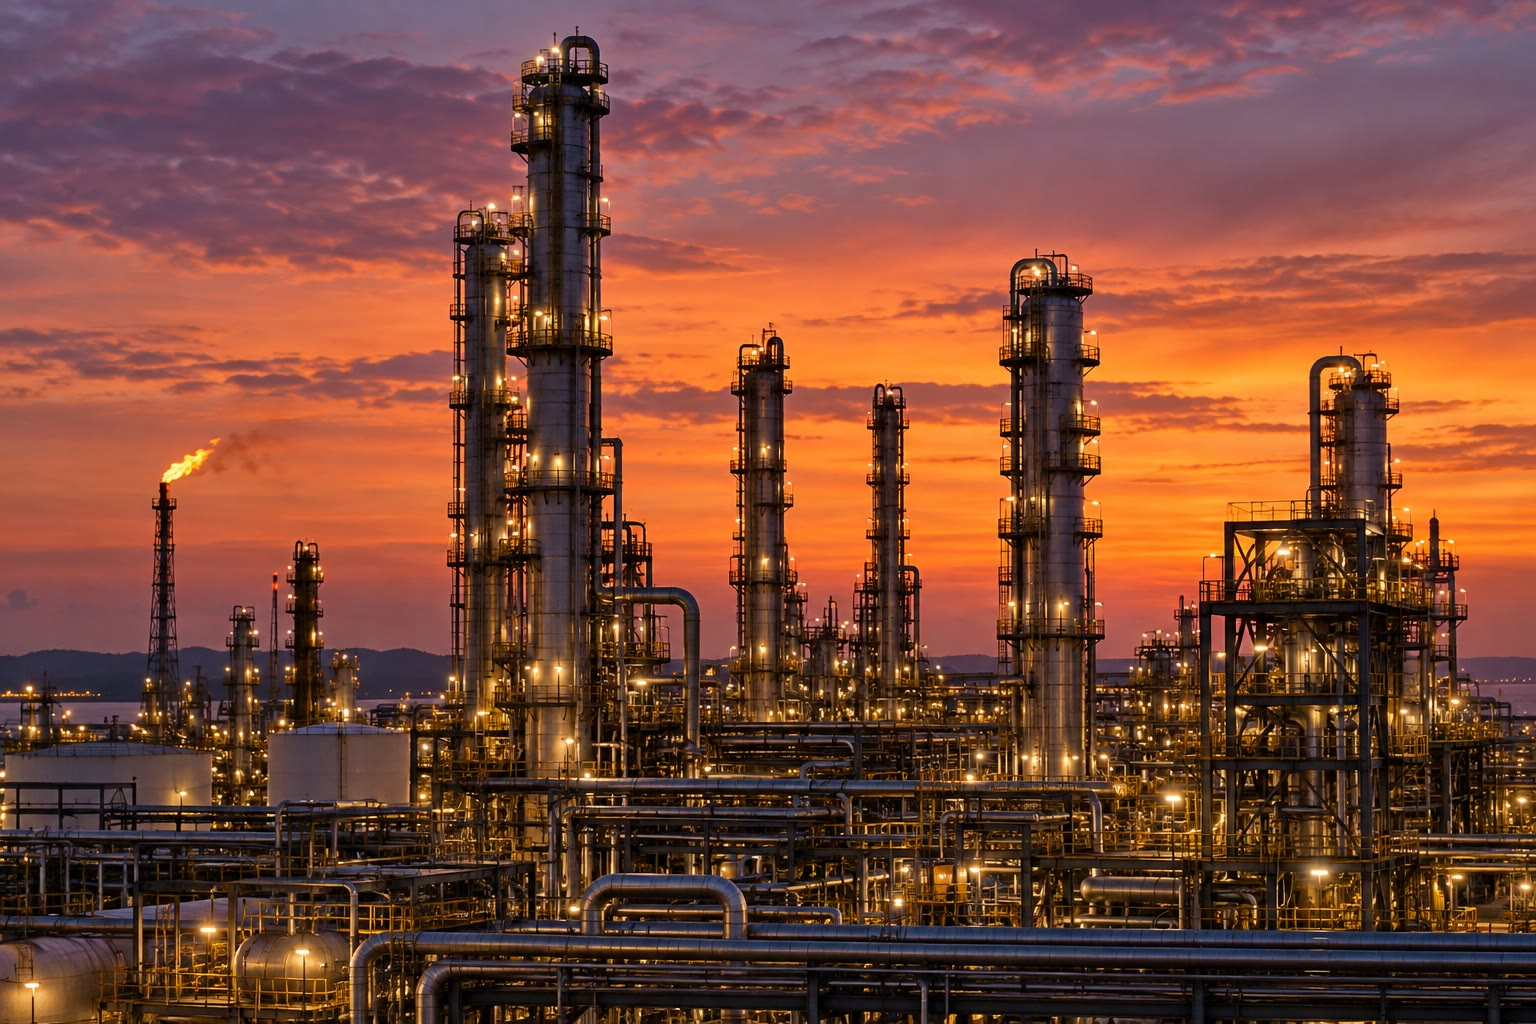
\includegraphics[width=0.52\linewidth]{images/book1/ai/g11-refinery-dusk.jpg}

{\small Kolom \omterm{def:g10:chemical-species:distillation}{distilasi} sebuah kilang minyak di senja hari.}
\end{omfigure}

\begin{safety}{\ghs[0.66cm]{GHS02}\ghs[0.66cm]{GHS04}\ghs[0.66cm]{GHS07}\ghs[0.66cm]{GHS08}\ghs[0.66cm]{GHS09}}
% ledger: ghs:butane, ghs:pentane
Butana adalah gas yang sangat mudah menyala, disimpan di bawah tekanan.
Pentana adalah cairan yang sangat mudah menyala; uapnya menimbulkan
kantuk, dapat merusak paru-paru jika tertelan, dan beracun bagi
kehidupan akuatik. Jangan ada nyala api di dekat \omterm{def:g11:organic-skeletons:alkane}{alkana} ringan; bekerja
di dalam lemari asam.
\end{safety}

\section{Latihan}


\begin{exercise}[$\star$]\label{exo:g11:organic-skeletons:1}
Berikan \omterm{def:g11:organic-skeletons:formulas}{rumus molekul} \omterm{def:g7:atoms-and-molecules:molecule}{molekul-molekul} yang digambar di sini, dan katakan
apakah keduanya \omterm{def:g11:organic-skeletons:isomer}{isomer}:
\setchemfig{atom sep=1.6em}
\chemfig{-[:30]-[:-30]-[:30]-[:-30]-[:30]} \quad dan \quad
\chemfig{-[:30](-[:90])-[:-30]-[:30]-[:-30]}.
\end{exercise}

\begin{exercise}[$\star$]\label{exo:g11:organic-skeletons:2}
Namailah: \ce{CH3-CH2-CH3}; \ce{CH3-CH2-CH2-CH2-CH2-CH3};
\chemfig{CH_3-CH(-[2]CH_3)-CH_2-CH_3}.
\end{exercise}

\begin{exercise}[$\star$]\label{exo:g11:organic-skeletons:3}
Tuliskan \omterm{def:g11:organic-skeletons:formulas}{rumus struktur ringkas} propana dan 2-metilpropana, dan \omterm{def:g11:organic-skeletons:formulas}{rumus
struktur} etana.
\end{exercise}

\begin{exercise}[$\star$]\label{exo:g11:organic-skeletons:4}
Hitunglah \omterm{def:g7:atoms-and-molecules:atom}{atom} karbon dan hidrogen setiap \omterm{def:g7:atoms-and-molecules:molecule}{molekul}:
\setchemfig{atom sep=1.6em}
\chemfig{-[:30]-[:-30](-[:-90])-[:30]-[:-30]} \quad dan \quad
\chemfig{*6(------)}.
\end{exercise}

\begin{exercise}[$\star$]\label{exo:g11:organic-skeletons:5}
Berikan \omterm{def:g11:organic-skeletons:formulas}{rumus molekul} \omterm{def:g11:organic-skeletons:alkane}{alkana} dengan 8 \omterm{def:g7:atoms-and-molecules:atom}{atom} karbon, dan banyaknya \omterm{def:g7:atoms-and-molecules:atom}{atom}
karbon \omterm{def:g11:organic-skeletons:alkane}{alkana} dengan 20 \omterm{def:g7:atoms-and-molecules:atom}{atom} hidrogen.
\end{exercise}

\begin{exercise}[$\star\star$]\label{exo:g11:organic-skeletons:6}
Gambarlah \omterm{def:g11:organic-skeletons:formulas}{rumus kerangka} 3-metilheksana, 2,2-dimetilbutana, dan
3-etilpentana, lalu berikan \omterm{def:g11:organic-skeletons:formulas}{rumus molekulnya}.
\end{exercise}

\begin{exercise}[$\star\star$]\label{exo:g11:organic-skeletons:7}
Gambarlah dan namailah ketiga \omterm{def:g11:organic-skeletons:isomer}{isomer} \ce{C5H12}.
\end{exercise}

\begin{exercise}[$\star\star$]\label{exo:g11:organic-skeletons:8}
Nama-nama berikut salah. Gambarlah setiap \omterm{def:g7:atoms-and-molecules:molecule}{molekul} dan berikan namanya
yang benar: 2-etilbutana; 4-metilpentana; 1-metilbutana.
\end{exercise}

\begin{exercise}[$\star\star$]\label{exo:g11:organic-skeletons:9}
Dengan gambar \omterm{def:g11:organic-skeletons:isomer}{isomer-isomer} \ce{C5H12}, urutkan \omterm{def:g11:organic-skeletons:isomer}{isomer-isomer} itu menurut
suhu didihnya dan jelaskan urutannya.
\end{exercise}

\begin{exercise}[$\star\star$]\label{exo:g11:organic-skeletons:10}
Sikloheksana adalah \ce{C6H12} dan heksana \ce{C6H14}. Jelaskan kedua
\omterm{def:g7:atoms-and-molecules:atom}{atom} hidrogen yang hilang itu. Apakah kedua senyawa itu \omterm{def:g11:organic-skeletons:isomer}{isomer}? Apakah
sikloheksana sebuah \omterm{def:g11:organic-skeletons:alkane}{alkana}?
\end{exercise}

\begin{exercise}[$\star\star$]\label{exo:g11:organic-skeletons:11}
Di antara propana, butana, 2-metilpropana, dan siklobutana (\ce{C4H8},
cincin empat \omterm{def:g7:atoms-and-molecules:atom}{atom} karbon), manakah yang saling berisomer?
\end{exercise}

\begin{exercise}[$\star\star\star$]\label{exo:g11:organic-skeletons:12}
Gambarlah dan namailah kelima \omterm{def:g11:organic-skeletons:isomer}{isomer} \ce{C6H14}.
\end{exercise}

\begin{exercise}[$\star\star\star$]\label{exo:g11:organic-skeletons:13}
Bayangkan \omterm{def:g11:organic-skeletons:alkane}{alkana} rantai lurus sebagai garis zig-zag yang panjang dan
\omterm{def:g11:organic-skeletons:alkane}{alkana} yang sangat bercabang sebagai bola. Dengan gambaran ini, jelaskan
mengapa percabangan menurunkan suhu didih \omterm{def:g11:organic-skeletons:isomer}{isomer-isomer}.
\end{exercise}

\begin{exercise}[$\star\star\star$]\label{exo:g11:organic-skeletons:14}
Namailah \omterm{def:g11:organic-skeletons:alkane}{alkana}
\begin{center}
\chemfig{CH_3-CH(-[2]CH_3)-CH_2-C(-[2]CH_3)(-[6]CH_3)-CH_2-CH_3}
\end{center}
\end{exercise}

\begin{exercise}[$\star\star\star$]\label{exo:g11:organic-skeletons:15}
Senyawa acuan untuk bensin, ``isooktana'', adalah
2,2,4-trimetilpentana. Gambarlah \omterm{def:g11:organic-skeletons:formulas}{rumus kerangkanya}, periksalah bahwa
senyawa itu \omterm{def:g11:organic-skeletons:isomer}{isomer} oktana, dan tuliskan \omterm{def:g11:organic-skeletons:formulas}{rumus struktur ringkasnya}.
\end{exercise}

\section{Soal: Gas Korek Api}

\begin{problem}[{Soal akhir pekan --- berapa banyak \omterm{def:g11:organic-skeletons:alkane}{alkana} berbeda yang
memiliki rumus \ce{C7H16}?}]
\label{pb:g11:organic-skeletons:1}
% ledger: bp:C3H8, bp:C4H10, bp:isobutane
Korek api gas berisi butana; tabung gas kemah untuk musim dingin berisi
\omterm{def:g6:pure-substances-and-mixtures:mixture}{campuran} yang lebih kaya propana atau 2-metilpropana. Butana mendidih
pada sekitar \qty{0}{\celsius}, 2-metilpropana pada
\qty{-11.7}{\celsius}, dan propana pada \qty{-42}{\celsius}.

\medskip
\noindent\textbf{Bagian I --- Dua gas dengan satu rumus.}
\begin{enumerate}
  \item Berikan \omterm{def:g11:organic-skeletons:formulas}{rumus molekul} butana, dan periksalah bahwa rumus itu
        sesuai dengan rumus umum \omterm{def:g11:organic-skeletons:alkane}{alkana}.
  \item Gambarlah \omterm{def:g11:organic-skeletons:formulas}{rumus strukturnya}.
  \item Tuliskan \omterm{def:g11:organic-skeletons:formulas}{rumus struktur ringkas} dan \omterm{def:g11:organic-skeletons:formulas}{rumus kerangkanya}.
  \item Gambarlah 2-metilpropana dengan ketiga cara yang sama. Mengapa
        \omterm{def:g11:organic-skeletons:formulas}{rumus molekulnya} sama?
  \item Apakah butana dan 2-metilpropana \omterm{def:g11:organic-skeletons:isomer}{isomer}? \omterm{def:g11:organic-skeletons:isomer}{Isomer} jenis apa?
\end{enumerate}

\medskip
\noindent\textbf{Bagian II --- Dalam \omterm{def:g4:air-a-mixture-of-gases:air}{udara} dingin.}
\begin{enumerate}[resume]
  \item Manakah di antara ketiga gas itu yang berupa gas pada
        \qty{20}{\celsius} dan tekanan normal?
  \item Sebuah korek api gas yang terbuka dipakai di luar ruangan pada
        \qty{-5}{\celsius}. Mengapa nyalanya buruk?
  \item Mengapa tabung gas untuk musim dingin kaya akan propana atau
        2-metilpropana?
  \item Jelaskan mengapa 2-metilpropana mendidih lebih rendah daripada
        butana.
  \item Mengapa propana tidak memiliki \omterm{def:g11:organic-skeletons:isomer}{isomer}?
\end{enumerate}

\medskip
\noindent\textbf{Bagian III --- Menamai dan menghitung.}
\begin{enumerate}[resume]
  \item Namailah \chemfig{CH_3-CH(-[2]CH_3)-CH_2-CH_3}.
  \item Mengapa nama ``3-metilbutana'' salah untuk \omterm{def:g7:atoms-and-molecules:molecule}{molekul} yang sama?
  \item Berapa \omterm{def:g11:organic-skeletons:isomer}{isomer} \omterm{def:g11:organic-skeletons:alkane}{alkana} yang memiliki rumus \ce{C4H10},
        \ce{C5H12}, dan \ce{C6H14}?
\end{enumerate}

\medskip
\noindent\textbf{Bagian IV --- \omterm{def:g11:organic-skeletons:isomer}{Isomer-isomer} \ce{C7H16}.}
\begin{enumerate}[resume]
  \item Gambarlah \omterm{def:g11:organic-skeletons:isomer}{isomer} rantai lurusnya dan namailah.
  \item Gambarlah dan namailah \omterm{def:g11:organic-skeletons:isomer}{isomer-isomer} yang rantai terpanjangnya
        memiliki enam \omterm{def:g7:atoms-and-molecules:atom}{atom} karbon. Mengapa tidak ada ``4-metilheksana''?
  \item Gambarlah dan namailah \omterm{def:g11:organic-skeletons:isomer}{isomer-isomer} yang rantai terpanjangnya
        memiliki lima \omterm{def:g7:atoms-and-molecules:atom}{atom} karbon dan dua gugus metil.
  \item Adakah \omterm{def:g11:organic-skeletons:isomer}{isomer} dengan rantai lima karbon dan satu gugus etil?
        Mengapa gugus etil itu hanya dapat terletak pada karbon 3?
  \item Gambarlah dan namailah \omterm{def:g11:organic-skeletons:isomer}{isomer} yang rantai terpanjangnya memiliki
        empat \omterm{def:g7:atoms-and-molecules:atom}{atom} karbon.
  \item Hitunglah semua \omterm{def:g11:organic-skeletons:isomer}{isomer} yang ditemukan.
  \item Nyatakan jawaban akhirnya: berapa \omterm{def:g11:organic-skeletons:isomer}{isomer struktur} yang dimiliki
        heptana, termasuk heptana itu sendiri?
\end{enumerate}
\end{problem}
